\documentclass[12pt]{amsart}
\usepackage{style}

\author{Blake Farman}
\address{Lafayette College}
\title[Final Exam]{Final Exam\\Math 161}
\date{December 13, 2018}

\begin{document}
\maketitle

\begin{center}
  \fbox{\fbox{\parbox{5.5in}{
        \noindent Answer the questions in the spaces provided on the
        question sheets and turn them in at the end of the exam period.
        You may \textbf{not} use a calculator or any other electronic device, including cell phones, smart watches, etc.\\

        \noindent 
        All supporting work is required.
        Unsupported or otherwise mysterious answers will \textbf{not receive credit.}
        It is advised, although not required, that you check your answers.\\
        
        \noindent By writing your name on the line below, you indicate that you have read and understand these directions.}}}
\end{center}

\vspace{0.2in}
\makebox[\textwidth]{Name:\enspace\hrulefill}
\vspace{0.2in}

\theoremstyle{definition}
\newtheorem{thm}{}
\renewcommand{\qedsymbol}{}

\[
\begin{array}{|c|c|c|}
  \hline
  \text{Problem} & \text{Points Earned} & \text{Points Possible}\\
  \hline
  1 & & 5\\
  \hline
  2 & & 3\\
  \hline
  3 & & 4\\
  \hline
  4 & & 10\\
  \hline
  5 & & 6\\
  \hline
  6 & & 6\\
  \hline
  7 & & 16\\
  \hline
  8 & & 10\\
  \hline
  9 & & 10\\
  \hline
  10 & & 10\\
  \hline
  11 & & 10\\
  \hline
  12 & & 10\\
  \hline
  \text{Total} & & 100\\
  \hline
\end{array}
\]

\newpage

\section*{Fill in the Blank}

\begin{thm}[5 Points - Derivative Rules]
  Let \(c\) be a constant.
  If \(f\) and \(g\) are differentiable functions, then
  \begin{enumerate}[(a)]
  \item
    \(\dfrac{\dif}{\dif x}\left(c\right) =\ \line(1,0){150}\)
    \vspace{.25in}
  \item
    \(\dfrac{\dif}{\dif x}\left(x^n\right) =\ \line(1,0){150}\)
    \vspace{.25in}
  \item
    \(\dfrac{\dif}{\dif x}\left(cf(x)\right) =\ \line(1,0){150}\)
    \vspace{.25in}
  \item
    \(\dfrac{\dif}{\dif x}\left(f(x) + g(x)\right) =\ \line(1,0){150}\)
    \vspace{.25in}
  \item
    \(\dfrac{\dif}{\dif x}\left(f(x) - g(x)\right) =\ \line(1,0){150}\)
    \vspace{.25in}
  \end{enumerate}
\end{thm}

\begin{thm}[3 Points]
  State the following:
  \begin{enumerate}[(a)]
  \item
    Product Rule:\\
    \[\dfrac{\dif}{\dif x}\left(f(x)g(x)\right) =\ \line(1,0){200}\]
    \vspace{.25in}
  \item
    Quotient Rule:\\
    \[\dfrac{\dif}{\dif x}\left(\dfrac{f(x)}{g(x)}\right) =\ \line(1,0){200}\]
    \vspace{.25in}
  \item
    Chain Rule:\\
    \[\dfrac{\dif}{\dif x}\left(f \circ g (x)\right) = \dfrac{\dif}{\dif x} f(g(x)) =\ \line(1,0){200}\]
    \vspace{.25in}
  \end{enumerate}
\end{thm}

\newpage

\begin{thm}[4 Points]
  Differentiate:
  \begin{enumerate}[(a)]
  \item
    \(\dfrac{\dif}{\dif x}e^x=\ \line(1,0){150}\)
    \vspace{.25in}
  \item
    \(\dfrac{\dif}{\dif x}\ln(x)=\ \line(1,0){150}\)
    \vspace{.25in}
  \item
    \(\dfrac{\dif}{\dif x}a^x=\ \line(1,0){150}\)
    \vspace{.25in}
  \item
    \(\dfrac{\dif}{\dif x}\log_a(x)=\ \line(1,0){150}\)  
  \end{enumerate}
\end{thm}


\begin{thm}[10 points - Integration]
  \begin{enumerate}[(a)]
  \item
    The Fundamental Theorem of Calculus, Part II:\\
    If \(f(x)\) is a continuous function on the interval \([a,b]\) and \(F(x)\) is any antiderivative of \(f(x)\), then\\ 
    
    \[\displaystyle{\int_a^bf(x)\dif x= }{\underline{\hspace{2in}}}\]

    \vspace{.5in}

  \item
    Let \(n\neq -1\) be a fixed number,\(\displaystyle{\int x^ndx=}\){\underline{\hspace{2in}}}

    \vspace{.25in}

  \item
    \(\displaystyle{\int \sin(x)dx=}\){\underline{\hspace{2in}}} 

    \vspace{.25in}

  \item
    \(\displaystyle{\int \cos(x)dx=}\){\underline{\hspace{2in}}} 

    \vspace{.25in}

  \item
    \(\displaystyle{\int \sec(x)\tan(x)dx=\ \line(1,0){150}}\)

    \vspace{.25in}

  \item
    \(\displaystyle{\int\sec^2(x)dx=\ \line(1,0){150}}\)

    \vspace{.25in}

  \item
    \(\displaystyle{\int\csc(x)\cot(x)dx=\ \line(1,0){150}}\)

    \vspace{.25in}

  \item
    \(\displaystyle{\int\csc^2(x)dx=\ \line(1,0){150}}\)

    \vspace{.25in}

  \item \(\displaystyle{\int e^xdx=}\){\underline{\hspace{2in}}} 

    \vspace{.25in}

  \item \(\displaystyle{\int\frac{1}{x}dx=}\){\underline{\hspace{2in}}} 
  \end{enumerate}
\end{thm}

\section*{Short Answer}

\begin{thm}[6 Points]
  Let \(\displaystyle{y=e^{x\sec x}}\).  Find the equation of the tangent line to the curve at \((0,1)\).
\end{thm}

\vspace{3in}

\begin{thm}[6 Points]
  Find the limit: \(\displaystyle{\lim_{x\rightarrow\infty}\left[\ln(1+ex)-\ln(x)\right]}\)
\end{thm}

\newpage


\begin{thm}[16 Points]
  Sketch the curve \(\displaystyle{f(x)=\frac{x^2}{x-4}}.\)
  \begin{enumerate}[(a)]
  \item
    Find the asymptotes.  Enter NONE if there are none. (Use calculus to justify your answer!)\\ \\ Horizontal:\hskip .5 truein \hrulefill\\ \\ Oblique:\hskip .5 truein \hrulefill\\\ \\ Vertical:\hskip .5 truein \hrulefill
    \vspace{1.2in}
  \item
    Find the intervals where the function is increasing and decreasing. Enter NONE if not applicable.\\ \\
    Increasing:\hskip .5 truein \hrulefill\\ \\ Decreasing:\hskip .5 truein \hrulefill
    \vspace{2in}
  \item
    State the local maximum and local minimum value(s). Enter NONE if not applicable.\\ \\
    Local maximum value(s):\hskip .5 truein \hrulefill\\ \\ Local minimum value(s):\hskip .5 truein \hrulefill
    \vspace{2in}
  \item
    Find the intervals on which the function is concave up and concave down. State the inflection points. Enter NONE if not applicable.\\ \\
    Concave Up:\hskip .5 truein \hrulefill\\ \\ Concave Down:\hskip .5 truein \hrulefill\\ \\ Inflection Points:\hskip .5 truein \hrulefill
    \vspace{2in}
  \item Use parts (a)-(d) to sketch the curve.  Be sure that your graph is labeled and neat. Messy/incoherent graphs will receive zero points.
    \begin{center}
      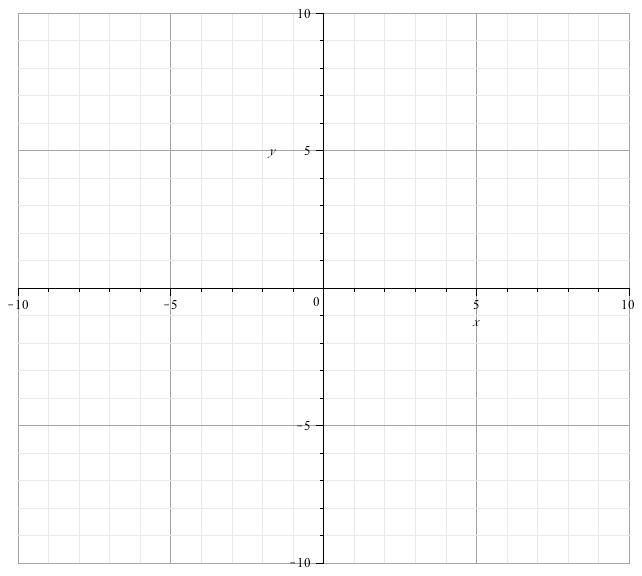
\includegraphics[scale=.75]{graphpaper}
    \end{center}
  \end{enumerate}
\end{thm}

\newpage

\begin{thm}[10 Points]
  A farmer has 2400 feet of fencing and wants to fence off a rectangular field that borders a straight river.  The farmer needs no fence along the river.  What are the dimensions of the field that has the largest area, and what is that largest area?
\end{thm}

\vspace{3in}

\begin{thm}[10 Points]
  Gas is escaping a spherical balloon at the rate of 4 \(cm^3\) per minute.  How fast is the surface area shrinking when the radius is 24 \(cm\)?  For a sphere, \(\displaystyle{V=\frac{4}{3}\pi r^3}\) and \(\displaystyle{S=4\pi r^2}\) where \(V\) is volume, \(S\) is surface area and \(r\) is the radius of the balloon.
\end{thm}

\newpage

\begin{thm}[10 Points]
  Evaluate the integral \(\displaystyle{\int \frac{e^x}{1+e^x}dx.}\)
\end{thm}

\vspace{3in}

\begin{thm}[10 Points]
  Find \(\displaystyle{\int_0^1 4x^3dx}\) using the definition and the identity
  \[\sum_{i=1}^n i^3 = \left(\frac{n(n+1)}{2}\right)^2 = \frac{n^2(n+1)^2}{4}.\]
\end{thm}

\newpage

\begin{thm}[10 Points]
  Evaluate the integral \(\displaystyle{\int_{0}^{\sqrt{\frac{\pi}{2}}}4x\cos(x^2)dx}.\)
\end{thm}

\end{document}



